\documentclass{article}
\usepackage[utf8]{inputenc}
\usepackage[portuguese]{babel}

\usepackage{listings}
\usepackage{color}
\usepackage{xcolor}
\usepackage{url}
 
\definecolor{codegreen}{rgb}{0,0.6,0}
\definecolor{codegray}{rgb}{0.5,0.5,0.5}
\definecolor{codepurple}{rgb}{0.58,0,0.82}
\definecolor{backcolour}{rgb}{0.95,0.95,0.92}
 
\lstdefinestyle{slstyle}{
    backgroundcolor=\color{backcolour},   
    commentstyle=\color{codegreen},
    keywordstyle=\color{magenta},
    numberstyle=\tiny\color{codegray},
    stringstyle=\color{codepurple},
    basicstyle=\footnotesize,
    language=C,
    morekeywords={*, sequence, instrument, performance, in, on, play, always, at, and, except, after, sequentially, times, loop, number},
    breakatwhitespace=false,         
    breaklines=true,                 
    captionpos=t,                    
    keepspaces=true,                 
    numbers=left,                    
    numbersep=5pt,                  
    showspaces=false,                
    showstringspaces=false,
    showtabs=false,                  
    tabsize=2
}
\lstset{style=slstyle}

\usepackage{caption}
\DeclareCaptionFont{white}{\color{white}}
\DeclareCaptionFormat{listing}{\colorbox{gray}{\parbox{\textwidth}{#3}}}
\captionsetup[lstlisting]{format=listing,labelfont=white,textfont=white}

\title{Especificação da Linguagem}
\author{Grupo 12, LFA}
\date{Junho 2018}

\usepackage{natbib}
\usepackage{graphicx}

\begin{document}
\def\titulo{Especificação da Linguagem}
\def\grupo{Grupo 12, LFA}
\def\empresa{Universidade de Aveiro}
\def\autores{António Santos\par Beatriz Borges\par Gustavo Inácio\par Filipe Vale\par Tomás Freitas\par}
\def\logotipo{ua.pdf}

%%%%%% CAPA %%%%%%
\begin{titlepage}
\begin{center}
%
\vspace*{40mm}
%
{\Huge \titulo}\\ 
%
\vspace{8mm}
%
{\Large \grupo}\\
%
\vspace{2mm}
%
{\Large \empresa}\\
%
\vspace{10mm}
%
{\LARGE \autores}
%
\vspace{30mm}
%
\begin{figure}[h]
\center
\includegraphics{\logotipo}
\end{figure}
%
\vspace{30mm}
\end{center}
\end{titlepage}

%%%%%% FIM CAPA %%%%%%


\maketitle

\tableofcontents
\clearpage

\section{Estruturas de dados (e tipos de variáveis)} \label{variables}
\subsection{Sequências}
Uma sequência de notas e silêncios pode ser definida, através da palavra chave \texttt{sequence}, como:
\begin{lstlisting} 
sequence melody = [C C G G A A G R F F E E D D C R]; // os espacos sao opcionais
\end{lstlisting}

\subsubsection{Notas musicais}
A notas são identificadas pela sua letra:
\begin{itemize}
    \item \texttt{C} para Dó,
    \item \texttt{D} para Ré,
    \item \texttt{E} para Mi,
    \item \texttt{F} para Fá,
    \item \texttt{G} para Sol,
    \item \texttt{A} para Lá,
    \item \texttt{B} para Si.
\end{itemize}
A letra \texttt{R} é usada para silêncios (derivada de \textit{Rests}).

Um cardinal (\texttt{\#}) a seguir à letra sobe a respetiva nota por meio tom; um b minúsculo (\texttt{b}) a seguir à letra desce a respetiva nota por meio tom. Mais que um \texttt{\#} ou \texttt{b} podem ser aplicados a uma nota (por exemplo, \texttt{C\#\#}).

Pode, depois do tom, aparecer um número, entre 0 e 8. Este especifica a oitava a usar, sendo 0 a mais grave e 8 a mais aguda. Por omissão, a quarta oitava é usada.

Assim, a sequência já apresentada podia reescrita da seguinte forma:
\begin{lstlisting} 
sequence melody = [C4 B# G G4 A4 A G R F E#4 Fb4 E D D4 C4 R];
\end{lstlisting}

Finalmente, uma sequência pode ser definida a partir doutra sequência:
\begin{lstlisting} 
sequence melody = [C C G G A A G R F F E E D D C R];

sequence r = [E G E melody D E D C]; // so e possivel utilizar esta nomenclatura se 'melody' for uma sequence
// equivalente a:
// sequence r = [EGE CCGGAAGR FFEEDDCR DEDC];
\end{lstlisting}


\subsubsection{Duração duma nota}
Por omissão, uma nota demora um tempo\footnote{Em termos musicais, uma semínima.}. A sua duração depende do \textit{tempo}, ou \texttt{BPM}\footnote{\textit{Beats Per Minute}}, da música. Esta configuração é explorada na secção \ref{config}.

Uma nota pode, no entanto, tocar mais ou menos tempo. Há duas formas de especificar a duração duma dada nota:
\begin{enumerate}
    \item \textbf{Por extensão.} A duração da nota é especificada através de chavetas (\texttt{\{} e \texttt{\}}), relativamente à duração unitária. Por exemplo, \texttt{C\{4\}} demora o quádruplo do tempo de \texttt{C}, e \texttt{C\{0.75\}} demora três quartos do tempo de \texttt{C}.
    \item \textbf{Notação simplificada.} Utilizam-se apóstrofos para reduzir a duração duma nota em metade, havendo uma correspondência direta com a duração das notas musicais convencionadas
    \footnote{Semínima (duração de 1), colcheia (duração de 1/2), semicolcheia (duração de 1/4), etc.}. 
    Por exemplo, \texttt{C'} demora metade do tempo de \texttt{C}, e \texttt{C''} apenas um quarto. 
\end{enumerate}

\subsubsection{Acordes}
O símbolo \texttt{|} é usado para tocar várias notas em simultâneo, numa só sequência.
Para tocar o acorde de Dó maior (C, E e G), na quarta oitava, podíamos então escrever:
\begin{lstlisting} 
sequence intro = [C|E|G];
\end{lstlisting}

\subsection{Performances}
A associação duma sequência musical com um instrumento representa um terceiro tipo de dados, uma \texttt{performance}:
\begin{lstlisting} 
sequence twinkle = [CC GG AA G{2} FF EE DD C{2}];
performance p = twinkle on guitar;

// ou, alternativamente, definindo a sequencia implicitamente
performance p = [CC GG AA G{2} FF EE DD C{2}] on guitar;
\end{lstlisting}

\subsection{Números}
Números (inteiros ou reais) são também suportados:
\begin{lstlisting} 
number num = 4;
\end{lstlisting}
Números podem também ser usados para referenciar um dado momento entre o início e o fim, inclusive, da peça musical. O início da peça é representado pelo número 0. 
\subsubsection{Operador de duração}
O operador \texttt{|}\textit{x}\texttt{|}, aceita um parâmetro (\textit{x}), do tipo sequence ou performance, e devolve um número igual à sua duração.
\begin{lstlisting} 
sequence intro = [R{4} C{4} G{4} C5{3.5} E|G|C5{.5} Eb|G|C5{8} C{4} G{4}]; // Strauss - Also Sprach Zarathustra - Intro (https://www.8notes.com/scores/7213.asp)
number endIntro = |intro|;
\end{lstlisting}

\subsection{Instrumentos}
Para tocar sequência musical é, naturalmente, necessário especificar que instrumento deve ser utilizado. Assim, para tocar \textit{Twinkle, Twinkle, Little Star} com uma piano, teríamos:
\begin{lstlisting} 
// definir a sequencia
sequence twinkle =  [CC GG AA G{2} FF EE DD C{2}];

// utilizando performances
performance p = twinkle on piano;
\end{lstlisting}

Vários instrumentos podem ser usados para tocar uma dada sequência.

Os instrumentos disponíveis são os seguintes:
\begin{itemize}
    \item \texttt{piano};
    \item \texttt{guitar};
    \item \texttt{violin};
    \item \texttt{cello};
    \item \texttt{bass};
    \item \texttt{drums}.
\end{itemize}
A criação de novos instrumentos é suportada, num ficheiro externo de tipo auxiliar, estando detalhada na secção \ref{config}. No ficheiro de tipo principal, não é possível definir ou redefinir novos instrumentos, sendo apenas possível usá-los como constantes pré-definidas.

\subsection{Arrays}
Um array é uma coleção de várias instâncias da mesma estrutura de dados. Suportam-se arrays de sequências, instrumentos, performances e números.

Um array pode ser definido de duas formas distintas:
\begin{lstlisting} 
// criar um array com 4 instrumentos - e necessario usar a palavra chave instrument para indicar que e um array de instrumentos
instrument[] band = [piano, guitar, bass, drums];

// outra forma de definir o mesmo array
instrument[] band = piano and guitar and bass and drums;

// criar um array com 3 performances
performance[] p = [
    [D{1.5} D{0.5}   E  D G F#{2}] on piano, 
    [D{1.5} D{0.5}   E  D A G{2}] on bass,
    [D{1.5} D{0.5}   D5 B G F# E] on guitar];
\end{lstlisting} 

Pode usar-se um array para criar outro. A palavra chave \texttt{and} anexa ao fim do array já existente o elemento ou elementos dados.

\begin{lstlisting} 
instrument[] band = [piano, guitar, bass, drums];

// definir arrrays a partir de outros arrays
instrument[] new_band = band and violin;
\end{lstlisting} 

Para arrays de números, o operador \texttt{a->b}, que devolve um array de inteiros de tipo \texttt{[a, a+1, ..., b-1, b]} pode também ser utilizado para gerar um array.
\begin{lstlisting}
start_times = 0->3;
// equivalente a:
//    start_times = [0, 1, 2, 3];
\end{lstlisting}

Para se aceder a um instrumento, a notação de parênteses retos, começando a contar no 0, é usada. A notação de intervalo, com dois pontos (\texttt{:}) é também suportada.
\begin{lstlisting} 
performance[] p = [
    [D{1.5} D{0.5}   E  D G F#{2}] on piano, 
    [D{1.5} D{0.5}   E  D A G{2}] on bass,
    [D{1.5} D{0.5}   D5 B G F# E] on guitar];
    
// aceder ao primeiro elemento
performance intro = p[0];

// exemplo da notacao de intervalo
performance[] q = p[0:1] and [C5{1.5} C5{0.5} B G A G{3}] on violin and p[2:];
\end{lstlisting}


\section{Geração de aúdio} \label{audio}
\subsection{Reprodução}
Para reproduzir uma performance, utiliza-se a palavra chave \texttt{play}:
\begin{lstlisting} 
// definir uma performance
sequence twinkle =  [CC GG AA G{2} FF EE DD C{2}];
performance p = twinkle on piano;

// reproduzir a performance
play p;

// alternativamente, definir a performance implicitamente
play twinkle on piano;

// ou definir a performance e a sequencia implicitamente
play [CC GG AA G{2} FF EE DD C{2}] on piano;
\end{lstlisting} 
\subsection{Modos de reprodução}
No exemplo anterior, não foi especificado quando começar a tocar a sequência. Por omissão, a sequência começa a ser tocada no início da peça (por outras palavras, no tempo 0).

Averiguemos os diferentes modos de reprodução:

\subsubsection{Simultâneo}
Por omissão, todas as sequências são tocadas começando no tempo 0. Se há mais que uma sequência a ser tocada, todas as sequências são tocadas em paralelo.

\begin{lstlisting} 
play [CC GG AA G{2} FF EE DD C{2}] on piano;

// e equivalente, em termos do som produzido no ficheiro final, a
play [CC RR RR G{2} FR RE DR C{2}] on piano;
play [RR GG AA RR RF ER RD RR] on piano;
\end{lstlisting}

Um outro exemplo de reprodução simultânea é o seguinte, que separa melodia e harmonia em duas performances diferentes:
\begin{lstlisting} 
// definir sequencias
sequence twinkle = [CC GG AA G{2} FF EE DD C{2}];
sequence twinkle_bass = [C|E|G{2} F|A|C{2} C|E|G{4} F|A|C C|E|G G|B|D C|E|G];

// tocar performances
play twinkle on guitar;
play twinkle_bass on guitar;
\end{lstlisting}

\subsubsection{Usando Números}
A palavra chave \texttt{at} indica um número específico no qual a performance deve começar, independentemente de haver outras performances a decorrer nesse momento. 
\begin{lstlisting} 
performance verse = [CC E{2} GG B{2} C5C5 GG C{4}] on violin;
performance chorus = [GAGA ABBA GEGE EBBE] on violin;

number chorusStart = |verse|;

// tocar performances
play verse;
at chorusStart play chorus;
\end{lstlisting}

Uma performance pode ser tocada em mais que um momento.
\begin{lstlisting} 
performance verse = [CC E{2} GG B{2} C5C5 GG C{4}] on violin;
performance chorus = [GAGA ABBA GEGE EBBE] on violin;

number chorusStart = 2*|verse|;
number otherTimeChorusStarts = 3.14*|verse|;

// tocar performances (chorus e tocada 2 vezes)
play verse;
at chorusStart play chorus;
at otherTimeChorusStarts play chorus;
\end{lstlisting}

\subsubsection{Repetição}
Há duas palavras chaves que permitem a repetição: o uso da palavra chave \texttt{times} permite repetir uma performance 0 ou mais vezes. \texttt{loop} permite repetir uma performance até ao fim da duração atual da peça (determinada pelo fim mais tardio de qualquer outra sequência até aí adicionada).
\begin{lstlisting} 
performance verse = [CC E{2} GG B{2} C5C5 GG C{4}] on violin;
performance chorus = [GAGA ABBA GEGE EBBE] on violin;
performance bass = [G|B|D{4} A|D|F#{4} G|B|D{4} A|D|F#{4}] on bass;

number chorusStart = 2*|verse|;

// tocar performances
play verse on piano 2 times;
at chorusStart play chorus;

loop bass; // repete ate ao fim da musica
\end{lstlisting}

\subsection{Uso de arrays}
Um array pode ser reproduzido de forma simultânea (forma utilizada por omissão) ou sequencialmente (através do uso da palavra chave \texttt{sequentially}).

\begin{lstlisting} 
// exemplo com sequencias
sequence[] melody_lines = [
    [D{1.5} D{0.5}   E  D G F#{2}], 
    [D{1.5} D{0.5}   E  D A G{2}],
    [D{1.5} D{0.5}   D5 B G F# E],
    [C5{1.5} C5{0.5} B  G A G{3}]];

play melody_lines /*sequentially*/ on piano; // descomentar sequentially para tocar melody_lines de forma sequencial
\end{lstlisting}

\begin{lstlisting} 
// exemplo com instrumentos
instrument[] band = [piano, guitar, bass, drums];

play melody_lines[0] /*sequentially*/ on band;
\end{lstlisting}

\begin{lstlisting} 
// exemplo com performances
performance[] perfors = [
    [D{1.5} D{0.5}   E  D G F#{2}] on piano, 
    [D{1.5} D{0.5}   E  D A G{2}] on bass,
    [D{1.5} D{0.5}   D5 B G F# E] on guitar];
    
play perfors /*sequentially*/;
\end{lstlisting}
No entanto, não é possível reproduzir diretamente um array de sequências num array de instrumentos. Isto é, por exemplo, não é possível fazer o seguinte:
\begin{lstlisting} 
// definir array de sequencias
sequence[] melody_lines = [
    [D{1.5} D{0.5}   E  D G F#{2}], 
    [D{1.5} D{0.5}   E  D A G{2}],
    [D{1.5} D{0.5}   D5 B G F# E],
    [C5{1.5} C5{0.5} B  G A G{3}]];

// definir array de instrumentos
instrument[] band = [piano, guitar, bass, drums];

play melody_lines /*sequentially*/ on band; // ilegal!!
\end{lstlisting}
Para se obter este tipo de resultados, têm que ser utilizadas instruções de repetição (ver secção \ref{flux}).

\subsection{Modulações}
Podem obter-se versões modificadas de sequências ou performances através dos operadores de modulação. Estes operadores devolvem uma nova sequência ou performance, alterada em algum aspeto (tom ou tempo) em relação a uma dada sequência  ou performance original, respetivamente.
\subsubsection{de Tom}
Pode mudar-se o tom de uma dada sequência ou performance através dos operadores \texttt{+} e \texttt{-}. A sequência ou performance devolvida será a sequência ou performance original com todas as suas notas subidas ou descidas \textit{n} meios-tons\footnote{Doze meios-tons constituem uma oitava.}.
\begin{lstlisting} 
// sequencia original
sequence s = [D{1.5} D{0.5} E D G F#{2}];

sequence s1 = s - 36; // diminuir a oitava por 3 (36 = 3*12)
// equivalente a dizer:
//    sequence s1 =  [D1{1.5} D1{0.5} E1 D1 G1 F#1{2}];

// mudar oitava da sequencia
sequence s5 = s + 12; // aumentar a oitava por 1 (12 = 1*12)
// equivalente a dizer:
//    sequence s5 =  [D5{1.5} D5{0.5} E5 D5 G5 F#5{2}];
\end{lstlisting}
\begin{lstlisting} 
// performance original
performance p = [D{1.5} D{0.5} E D G F#{2}] on bass;

play p+5;
// equivalente a:
//    play  [F#{1.5} F#{0.5} G# F# B A#{2}] on bass;
\end{lstlisting}

\subsubsection{de Tempo}
Pode mudar-se o tempo (ou seja, a velocidade) de um dada sequência ou performance através dos operadores \texttt{*} e \texttt{/}. A sequência ou performance devolvida será a sequência ou performance original com todas as suas notas aceleradas ou atrasadas \textit{n} vezes.\footnote{A nova velocidade é dada por \texttt{velocidade original * fator}, ou por \texttt{velocidade original / fator}, conforme os operadores \texttt{*} ou \texttt{/} são usados, respetivamente.}
\begin{lstlisting} 
// performance original
performance p = [D{1.5} D{0.5} E D G F#{2}] on bass;

play p * 5; // toca a sequencia 5x mais rapido (cada nota dura 1/5 do seu tempo original)
// equivalente a:
//    play  [D{.3} D{0.1} E{.2} D{.2} G{.2} F#{.4}] on bass;
\end{lstlisting}

\begin{lstlisting} 
// performance original
performance p = [D{1.5} D{0.5} E D G F#{2}] on bass;

play (p + 5) * 5; // toca a sequencia 5x mais rapido, com todas as notas 5 meios-tons mais agudas
// equivalente a:
//    play  [F#{.3} F#{0.1} G#{.2} F#{.2} B{.2} A#{.4}] on bass;
\end{lstlisting}

\section{Interação com o exterior} \label{exterior}
\subsection{Estruturas de dados auxiliares}
\subsubsection{Strings}
Strings são sequências de caracteres, números e símbolos delimitadas por aspas (\texttt{"}).

Não existe um tipo de dados String explícito, sendo este usado apenas como parâmetro opcional para funções de I/O.
\subsection{getInt( string? )}
\texttt{getInt()} permite obter um inteiro através do \textit{Standard In}. 

Opcionalmente, pode ser passada uma String, que será impressa antes de aguardar a resposta do utilizador (uma String de \textit{prompt}).


\section{Controlo de fluxo} \label{flux}
\subsection{Instruções condicionais}
\subsubsection{if}
As palavras chave \texttt{if}, \texttt{else if} e \texttt{else} permitem testar condições. Os operadores suportados numa condição são os de igualdade (\texttt{==}), desigualdade (\texttt{!=}), menor (\texttt{<}), maior (\texttt{>}), menor ou igual (\texttt{<=}), e maior ou igual (\texttt{>=}).
\begin{lstlisting} 
sequence s = getSequence("Enter a sequence: ");

if (|s| > 5) {
    play s on piano;
} else if (|s| > 2) {
    play s on cello;
} else {
    play s on guitar;
}
\end{lstlisting}

\subsection{Intruções de repetição}
\subsubsection{for}
As palavras chave \texttt{for} e \texttt{in} permitem definir instruções de repetição, ou seja, permitem que um dado código seja executado múltiplas vezes, iterando sobre todos os elementos de um dado array.
\begin{lstlisting} 
// instrumentos 
instrument[] band = [piano, guitar, bass, drums];
for instrument inst in band {
    play [ABCDCBA] on inst;
}

// sequencias
sequence[] sequences = [
    [D{1.5} D{0.5}   E  D G F#{2}], 
    [D{1.5} D{0.5}   E  D A G{2}],
    [D{1.5} D{0.5}   D5 B G F# E],
    [C5{1.5} C5{0.5} B  G A G{3}]];
    
for sequence seq in sequences {
    play seq on piano;
}
    
// performances
performance[] perfors = [
    [D{1.5} D{0.5}   E  D G F#{2}] on piano, 
    [D{1.5} D{0.5}   E  D A G{2}] on bass,
    [D{1.5} D{0.5}   D5 B G F# E] on guitar];
    
number t = 0;
for performance perfor in perfors {
    at t play perfor;
    t = t + |perfor|;
}

// numeros
start_times = [0, 1, 3, 7];
for number t in start_times {
    at t play [C1 E1 G1 E1] on piano;
}
\end{lstlisting}

Caso se pretenda iterar sobre algum código um dado número de vezes, sem haver correspondência direta entre esse número e o conteúdo de um dado array, pode usar-se números num dado intervalo, usando o operador \texttt{a->b} (que devolve um array de inteiros de tipo \texttt{[a, a+1, ..., b-1, b]}):
\begin{lstlisting} 
instrument[] band = [piano, guitar, bass, drums];
sequence[] sequences = [
    [D{1.5} D{0.5}   E  D G F#{2}], 
    [D{1.5} D{0.5}   E  D A G{2}],
    [D{1.5} D{0.5}   D5 B G F# E],
    [C5{1.5} C5{0.5} B  G A G{3}]];

number t = 0;
for number i in 0->3 {
    at t play sequences[i] on band[i];
    t = t + |sequences[i]|;
}
\end{lstlisting}

\section{Configurações (ficheiro auxiliar)} \label{config}
Um ficheiro do tipo principal (ficheiros com extensão \texttt{.mux}) suporta um todas as operações descritas até este ponto. 
Várias configurações podem ser feitas no ficheiro auxiliar (ficheiros com extensão \texttt{.aux}). Nesta secção, vamos abordar as diferentes configurações que podem ser definidas através do ficheiro auxiliar.
\subsection{BPM (Beats Per Minute)}
\texttt{BPM} é uma palavra reservada\footnote{BPM não pode ser usado como nome de uma variável.} usada para configurar o \textit{tempo} da música. A configuração deve ser feita no ficheiro de configuração, mas é possível reescrevê-la no ficheiro principal (o que define a música a gerar).
\begin{lstlisting} 
BPM = 160;
\end{lstlisting}

\subsection{Especificação de (novos) instrumentos}
O formato \textit{midi} suporta 128 instrumentos diferentes\footnote{Para obter mais informação sobre os diferentes instrumentos disponíveis, ver \url{https://www.midi.org/specifications/item/gm-level-1-sound-set}.}.

É possível criar novos instrumentos associando a uma palavra um número, através da palavra chave \texttt{instrument}. O nome dado ao instrumento deixa de poder ser usado como nome de variável.

\begin{lstlisting} 
// definir dois novos instrumentos
instrument strings: 49;
instrument synth1: 81;
\end{lstlisting}

Os instrumentos já definidos estão associados aos seguintes códigos: 1(\texttt{piano}), 25(\texttt{guitar}), 41(\texttt{violin}), 43(\texttt{cello}), 44(\texttt{bass}), e 119(\texttt{drums}). 

É também possível definir novos instrumentos à custa de instrumentos já existentes, e associar nomes a tons.

\begin{lstlisting} 
// duplicar um instrumento ja existente
instrument percussion: drums;

// mapear tons (associar nomes a tons)
acousticBassDrum = B0;
bassDrum1 = C1;
sideStick = C#1;
acousticSnare = D1;
handClap = D#1;
electricSnare = E1;
lowFloorTom = F1;
closedHiHat = F#1;
highFloorTom = G1;
pedalHiHat = G#1;
lowTom = A1;
openHiHat = A#1;
lowMidTom = B1;
hiMidTom = C2;

// a um tom podem ser associados varios nomes
// (mas a um nome nao podem ser associadas mais que um tom)
LongWhistle = C4;
MiddleC = C4;
                     	 
\end{lstlisting}	 
É ainda possível criar um instrumento juntando vários instrumentos já existentes. Associa-se a uma nota (ou a um conjunto de notas, sendo o intervalo representado por \texttt{NotaInicial - NotaFinal}, incluindo os extremos) o instrumento que deve ser utilizado para a tocar, utilizando o operador \texttt{->}.

Se uma nota for definida mais que uma vez, a última definição será a usada. Se uma nota não for definida, gerará um erro se for reproduzida.
\begin{lstlisting} 
// definir um novo instrumento a partir de instrumentos existentes
instrument thing: B0-C4 -> drums,
                  G4 -> guitar,
                  A4-G5 -> guitar, 
                  C5-A8 -> piano; // notas C5-G5 redifinidas
\end{lstlisting}


\section{Especificação da linguagem destino} \label{target}
\subsection{Linguagem destino}
A linguagem destino do compilador foi Python 3, porque permite um maior foco na linguagem e no compilador, uma vez que facilita a manipulação de ficheiros do tipo MIDI através da biblioteca MIDIUtil.

Na geração de código utiliza-se, para cada performance, uma lista bastante detalhada, que permite a inserção modular de qualquer sequência de notas musicais ou acordes, suportando um número arbitrário de repetições e uma grande flexibilidade no tempo de inicio de reprodução da performance. Esta lista é parâmetro de entrada da função \textit{addnotes} que permite a inserção das notas, com os instrumentos certos no sítio certo da timeline. Uma lista exemplo é a seguinte:

\begin{lstlisting}
toadd = [[1,10,15,25,36], [(64,0.5,2,3),(62,0.25,25,4)], 3];
\end{lstlisting}

O primeiro elemento da lista é um \textit{Array} com os start times da performance. No exemplo acima, o array implica que a performance comece a tocar nos segundos 1, 10, 15, 25 e 36. Ainda no mesmo exemplo, o segundo elemento representa a descrição das notas que são \texttt{tuplos} constituídos da seguinte maneira: (nota, duração, instrumento, tempo de entrada relativo ao start time). O último elemento é o número de vezes que a performance é repetida em cada momento de inserção (com 5 start times, a performance será reproduzida 15 vezes).

\clearpage

\section{Exemplos} \label{example}
\subsection{Parabéns}
\begin{lstlisting}[caption=bday.aux]
// set default BPM setting
BPM = 200;
\end{lstlisting}

\begin{lstlisting}[caption=bday.mux]
// get user input
number repeat_times = getInt("Number of repetitions: ");

// define melody sequences
sequence[] melody_lines = [
    [D{1.5} D{0.5}   E  D G F#{2}], 
    [D{1.5} D{0.5}   E  D A G{2}],
    [D{1.5} D{0.5}   D5 B G F# E],
    [C5{1.5} C5{0.5} B  G A G{3}]];

// perform
number offset = 0;
for number n in 1->repeat_times {
	at offset play melody_lines + 12*(n-1) on piano sequentially;
	for sequence melody in melody_lines {
		offset = offset + |melody|;
	}
}
\end{lstlisting}

\clearpage
\subsection{Stromae - Alors on Danse}
\begin{lstlisting}[caption=rap.mux]
sequence alors = [G#2{.5}R{.5} C#3{.5}R{.5} G#3{1.2}G#3{1.2}G#3{.8} E3{.5}R{.5} A3{.5}R{.5} Eb3{1.2}Eb3{1.2}Eb3{.8}] + 12;
sequence alors2 = [E3 R{.33} E3 R{.33} E3 R{.33} E3 R{.33} E3 R{.33} E3{.5} F#3{.5} R{.1} Eb3{.5}R{.5} Eb3{.5}R{.5}Eb3{.5}]+ 24;

performance p_alors = alors on piano;

//play alors on piano;

at 2* |alors| play alors2 on piano;
at 3 * |alors| play alors2 on piano;
loop p_alors;

\end{lstlisting}


O compilador é robusto e flexível, suportando a ausência do ficheiro auxiliar. Nesse caso, o compilador assume uma configuração o equivalente ao seguinte ficheiro auxiliar:
\begin{lstlisting}[caption=default.aux]
BPM = 120;
\end{lstlisting}

\clearpage
\subsection{Stranger Things Theme}

\begin{lstlisting}[caption=StrangerThings.aux]
BPM = 160;

//definicao dos instrumentos a usar pela track
instrument vibrofone    : 12;
instrument synth        : 39;
instrument synthPiano   : 3; 
instrument slapBass	    : 37;
instrument harpsiChord	: 7;

\end{lstlisting}

\begin{lstlisting}[caption=StrangerThings.mux]
//Parte 1

sequence intro1 = [B4{0.25} E5{0.25} G5{0.25} B5{0.25} C6{0.25} B5{0.25} G5{0.25} E5{0.25}];
sequence intro2 = [R{0.25} B4{0.25} B4{0.25} B4{0.25} B4|C5{0.25} B4{0.25} B4{0.25}];
sequence intro3 = [R{0.5} G4{0.25} R{0.25}];
sequence intro4 = [E4{0.25}];

play intro1 on vibrofone 4 times;
play intro2 on synth 4 times;
play intro3 on synth 8 times;
play intro4 on synth 32 times;

//Parte 2
number parte2 = 4*|intro1|;

sequence bouncer = [C4''R'' E4''R'' G4''R'' B4''R'' C5''R'' B4''R'' G4''R'' E4''R''];
sequence ticker1  = [C3''R''C3''R{1.25}];
sequence ticker2  = [E3''R''E3''R{1.25}];

at parte2 play bouncer on slapBass 30 times;
at parte2 play bouncer on synthPiano 30 times;
at parte2 play ticker1 on slapBass 8 times;

number t1 = parte2 + 8*|ticker1|;
at t1 play ticker2 on slapBass 8 times;

sequence danglingNotes1 = [C5''R{1.75} G5''];
number t2 = t1 + 8*|ticker2|;
at t2 play danglingNotes1 on harpsiChord;
at t2 play ticker1 on slapBass 7 times;

sequence ticker3 = [D3''R''D3''R{1.25}];
sequence danglingNotes2 = [D4''R''D4''R{1.25} E4''R{3.75} E3''R{9.75}G4''R''G4''R{1.25}C4''];
number t3 = t2 + 7*|ticker1|;

at t3 play danglingNotes2 on harpsiChord;
at t3 play ticker3 on slapBass;

number t4 = t2 + 8*|ticker1|;
number t5 = t4 + 7*|ticker1|;

at t4 play ticker2 on slapBass 7 times;
at t5 play [G3''R''G3''] on slapBass;


sequence ticker10 = [C3''R''C3''R''];
number t6 = t4 + 8*|ticker1|;
at t6 play ticker1 on slapBass 6 times;
at t6 play ticker10 on synth 12 times;

number t7 = t6 + 12*|ticker10|;
sequence ticker4 = [D3''R'' D3''R'' R{0.5}C3''R'' C3''R''C3''R'' R{0.5}B2''R''];
sequence ticker5 = [D3''R'' D3''R'' C3''R''C3''R''C3''R''C3''R'' B2''R''B2''R''];
at t7 play ticker4 on slapBass;
at t7 play ticker5 on synth;


sequence ticker6 = [B2''R''B2''R''R];
sequence ticker7 = [B2''R''B2''R''];
number t8 = t7 + |ticker4|;
at t8 play ticker6 on slapBass 12 times;
at t8 play ticker7 on synth 24 times;


number t9 = t8 + 12*|ticker6|;
at t9 play ticker1 on slapBass 8 times;
at t9 play ticker1 on synth 8 times;
at t9 play [C5''R{1.75}G5''R{1.75}C5''R{7.75}D5''R{1.25}C5''R{1.25} B4|E4''] on harpsiChord;

number t10 = t9 + |ticker1|;
at t10 play [G3''R'']on synth 26 times;

\end{lstlisting}

\clearpage
\subsection{John Chambers - Beethoven's Favourite Waltz}
\begin{lstlisting}[caption=waltz.aux]
BPM = 320;

instrument flute: 74;
instrument strings: 45;
\end{lstlisting}

\begin{lstlisting}[caption=waltz.mux]
// beethoven's favourite waltz

sequence waltz = [
	B C5 

	D5 B G{2} B C5
	D5 B G{2} G5 F5 
	E5{2} E5{2} E5{2}
	E5{3} D5 C5 B

	A{2} A{2} A{2}  
	D5{3} C5  C5 A 
	G F G B A F 
	G4 D5 F5

	G5{2} G5{2} A5{2}  
	G5{2} G5{2} A5{2} 

	G5{2} A5{2} B5{2} 
	A5 F5 D5{2} E5 F5 

	G5 F5 G5 D5 F5 D5  
	G5 F5 G5 D5 F5 D5  
	G5{2} D5 C5 B A 
	G4 G B

	D5{2} D#5 C5 D5 C5  
	D5 B E5 D5 C5 B 
	A{2} A{2} D5{2}  
	B{2} R{2} G B

	D5{2} D5 C#5 D5 C5 

	D5 BE5 D5 C5 B 
	A{2} A G A B 
	G4 D5{2}

	G5{2} G5{2} B5 G5  
	D5{2} D5 G5 D5 B 
	G{2} G F G B 
	B{2} A{2} D5 F5

	G5{2} G5{2} B5 G5  
	D5{2} D5{2} G5 D5  
	B D5 G B A F 
	G{4}
];

at 2 play waltz + 12 on piano;
at 1 play waltz on flute;
play waltz - 24 on bass;

loop [G0 B0 D1] on strings; // simple bassline
\end{lstlisting}

\clearpage
\subsection{Alexandre Desplat - Courtyard Apocalypse}
\begin{lstlisting}[caption=court.aux]
BPM = 240;

instrument taiko : 117;

instrument synth : piano;
instrument synth : C2-G#2 -> taiko;

beat = F2;
\end{lstlisting}
\begin{lstlisting}[caption=court.mux]
//synth parte 1
sequence s1 = [C4C4A#3A#3C4C4F4F4];
sequence s2 = [D#4D#4D4D4D#4D#4G4G4];
sequence s3 = [F4F4D#4D#4F4F4];
sequence s4 = [G#4G#4G4G4G#4G#4D#5D#5];
sequence s5 = [G#4G#4G4G4G#4G#4C5C5];
sequence s6 = [G#4G#4G4G4G#4G#4A#4A#4];
sequence s7 = [G4G4F4F4G4G4C5C5];
sequence s8 = [G4G4F4F4G4G4G#4G#4G#4G#4G4G4G#4G#4F5F5G#4G#4G4G4G#4G#4F5F5G#4G#4G#4G#4G#4G#4G#4G#4G#4G#4G#4G#4G#4G#4G#4G#4];

play s1 on synth 4 times;
at 4*|s1| play s2 on synth 2 times;
at 4*|s1| + 2*|s2| play s3 on synth;

number t1 = 4*|s1| + 2*|s2| + |s3|;
at t1 play [A#4A#4] on synth;

performance ps1 = [A#4A#4] on synth;

number t2 = t1 + |ps1|;
at t2 play s3 on synth;

number t3 = t2 + |s3|;
at t3 play [G4G4] on synth;


performance ps2 = [G4G4] on synth;

number t4 = t3 +|ps2|;
at t4 play s5 on synth 2 times;
number t5 = t4 + 2*|s5|;
at t5 play s4 on synth;
number t6 = t5 + |s4|;
at t6 play s6 on synth;
number t7 = t6 + |s6|;
at t7 play s7 on synth;
number t8 = t7 + |s7|;
at t8 play s8 on synth;


//synth parte 2

number tl1 = 62;
sequence pl1 = [G3G3G#3G#3G#3G#3G#3G#3G#3G#3G#3G#3G#3G#3G#3G#3];
at tl1 play pl1 on synth 2 times;
number tl2 = tl1 + 2*|pl1|;
sequence pl2 = [A#3A#3G3G3G3G3G3G3G3G3G3G3G3G3G3G3];
at tl2 play pl2 on synth;
number tl3 = tl2 + |pl2|;
sequence pl3 = [D#3D#3F3F3F3F3F3F3F3F3F3F3F3F3F3F3F3F3];
at tl3 play pl3 on synth;
number tl4 = tl3 + |pl3|;
sequence pl4 = [C4C4C4C4C4C4C4C4C4C4C4C4C4C4C4C4];
at tl4 play pl4 on synth;

//synth de C2-G#2 -> taiko

performance p1 = [beat RR beat beat RRR beat RR beat beat RRR] on synth;
performance p2 = p1 + 3;
performance p3 = p1 - 5;
performance p4 = p1 - 4;
number n1 = |p1|;
number n2 = n1 + |p2|;
number n3 = n2 + |p3|;
number n4 = n3 + |p4|;
number n5 = n4 + |p1|;
number n6 = n5 + |p2|;
number n7 = n6 + |p3|;

play p1;
at n1 play p2;
at n2 play p3;
at n3 play p4;
at n4 play p1;
at n5 play p2;
at n6 play p3;
at n7 play p1;
\end{lstlisting}

\clearpage
\subsection{Mais exemplos}
No repositório do projeto, podem ser encontrados mais exemplos, na pasta \texttt{Visitor/examples/}.

Destaca-se o exemplo da música Despacito (\texttt{despacito.mux} e \texttt{despacito.aux}), que faz uso de 15 instrumentos, incluindo uma grande amostra de diferentes sons de percussão. Abaixo encontra-se uma imagem de um excerto do ficheiro MIDI gerado:

\begin{figure}[h]
    \center
    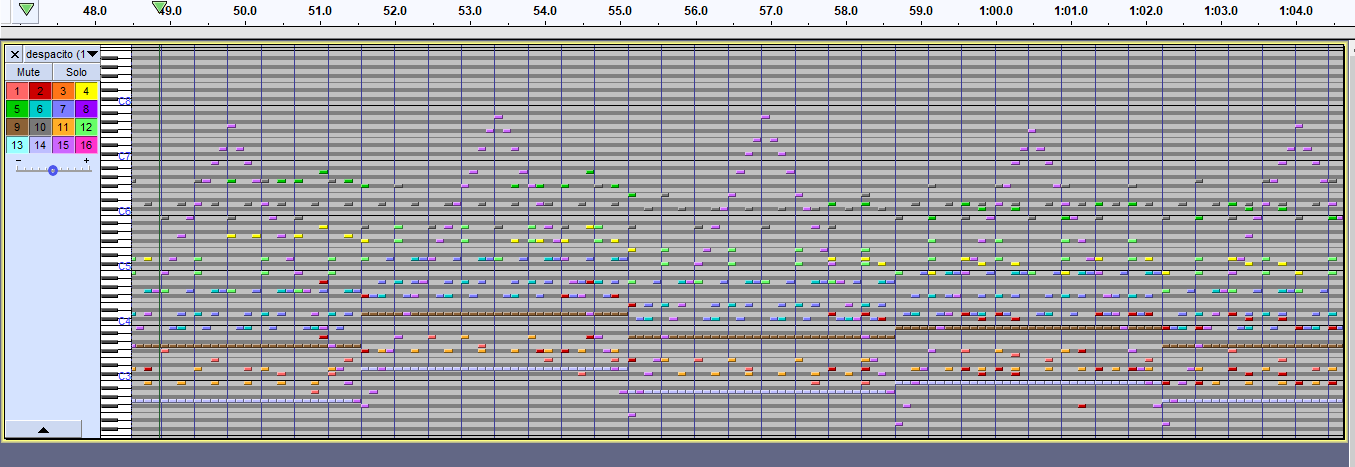
\includegraphics[width=\textwidth]{LFA-Final/despacito.png}
    \caption{Excerto do ficheiro gerado por \texttt{despacito.mux} e \texttt{despacito.aux}}
    \label{fig:my_label}
\end{figure}

\end{document}
